\documentclass[12pt, letterpaper]{article}
\usepackage[top=2.5cm, bottom=2.5cm, left=3cm, right=2.5cm]{geometry}
\usepackage[utf8]{inputenc}
\usepackage[T1]{fontenc}
\usepackage{lmodern}
\usepackage{amsmath, amssymb}
\usepackage{booktabs}
\usepackage{tabularx}
\usepackage{longtable}
\usepackage{array}
\usepackage{multirow}
\usepackage{xcolor}
\usepackage{graphicx}
\usepackage{float}
\usepackage{listings}
\usepackage[most, breakable]{tcolorbox}
\usepackage{enumitem}
\usepackage{fancyhdr}
\usepackage{titlesec}
\usepackage{setspace}
\usepackage{microtype}
\usepackage[hidelinks]{hyperref}
\usepackage{parskip}
\usepackage{pgfplots}
\pgfplotsset{compat=1.15}
\usepackage{tabularx}
\usepackage{booktabs}
\usepackage{float}

\usepackage{geometry}
\geometry{margin=1in}
% Colours
\definecolor{econblue}{RGB}{31,78,121}
\definecolor{researchgreen}{RGB}{21,101,45}
\definecolor{exampleorange}{RGB}{180,80,20}
\definecolor{lightgray}{RGB}{245,245,245}
\definecolor{boxblue}{RGB}{220,235,248}

% Section headings
\titleformat{\section}{\large\bfseries\color{econblue}}{\thesection}{1em}{}%
  [\vspace{-4pt}\rule{\linewidth}{0.4pt}]
\titleformat{\subsection}{\normalsize\bfseries\color{econblue}}{\thesubsection}{1em}{}
\titleformat{\subsubsection}{\normalsize\bfseries}{\thesubsubsection}{1em}{}

% Page style
\pagestyle{fancy}
\fancyhf{}
\fancyhead[L]{\small\itshape ECON 230 --- Introduction to Behavioural Economics}
\fancyhead[R]{\small\itshape Chapter 4: Today vs Tomorrow}
\fancyfoot[C]{\small\thepage}
\renewcommand{\headrulewidth}{0.4pt}
\setlength{\headheight}{14pt}

% tcolorbox styles
\tcbuselibrary{breakable, skins, listings}

\newtcolorbox{researchbox}{
  enhanced, breakable,
  colback=researchgreen!6, colframe=researchgreen!55,
  title=\textbf{Research Study},
  fonttitle=\bfseries\small,
  attach boxed title to top left={yshift=-2mm, xshift=6mm},
  boxed title style={colback=researchgreen!55, colframe=researchgreen!55},
  before upper={\setlength{\parskip}{4pt}}
}

\newtcolorbox{examplebox}[1]{
  enhanced, breakable,
  colback=exampleorange!6, colframe=exampleorange!45,
  title=\textbf{#1}, fonttitle=\bfseries\small
}

\newtcolorbox{keybox}{
  enhanced, colback=boxblue, colframe=econblue!70,
  fontupper=\small
}

% ASCII figure style
\lstset{
  basicstyle=\scriptsize\ttfamily,
  breaklines=false,
  keepspaces=true,
  columns=flexible,
  frame=single,
  backgroundcolor=\color{lightgray},
  xleftmargin=4pt, xrightmargin=4pt,
  aboveskip=6pt, belowskip=6pt
}

% Lists
\setlist[itemize]{leftmargin=1.5em, itemsep=2pt, topsep=4pt}
\setlist[enumerate]{leftmargin=1.5em, itemsep=2pt, topsep=4pt}
\onehalfspacing

\newcolumntype{Y}{>{\raggedright\arraybackslash}X}

\begin{document}

\begin{titlepage}
\centering\vspace*{3cm}
{\Large\bfseries\color{econblue} ECON 230 --- Introduction to Behavioural Economics\\[1em]}
{\large\bfseries Course Textbook\\[2em]}
{\LARGE\bfseries\color{econblue} Chapter 4\\[0.5em]}
{\Large\bfseries Today vs Tomorrow --- Time Inconsistency and Present Bias\\[2em]}
\vfill
{\normalsize University of Northern British Columbia\\
Instructor: Prof.\ Muhebullah Karimzada\\
Term: Winter 2027}
\end{titlepage}
\tableofcontents
\newpage


\medskip


\section*{Chapter Overview}
\addcontentsline{toc}{section}{Chapter Overview}


Chapters 1 through 3 examined how people make decisions under risk and uncertainty. This chapter turns to a different dimension of decision-making: time. Specifically, it asks why people so reliably fail to follow through on their own plans. Why do gym memberships purchased in January sit idle by March? Why do most people save far less than they intend to? Why does the student who plans to start their essay this week end up writing it the night before the deadline --- every time?

The standard economic model has a tidy answer: people discount the future at a constant rate, patiently weighing present costs against future benefits according to a stable preference ordering. The uncomfortable empirical reality is that this model is systematically wrong in ways that matter enormously --- for individual welfare, for retirement security, for public health, and for a wide range of policy interventions.

The culprit is \textbf{present bias}: the tendency to weight payoffs received in the immediate present disproportionately relative to payoffs received at any point in the future, even the near future. Present bias is not the same as simply being impatient --- a person can be very patient in the long run yet still be powerfully pulled toward the immediate option when it becomes available. This asymmetry between \textit{when decisions are made} (in the future, when everything is distant) and \textit{when they are executed} (in the present, when temptation is near) generates \textbf{time inconsistency}: the systematic reversal of preferences as the future becomes the present.

This chapter develops the theory of present bias and time inconsistency from first principles. We begin with the standard model of exponential discounting and its key property of time consistency, then examine the empirical evidence showing that people's discount rates are not constant but declining, then introduce hyperbolic discounting and its tractable approximation, the \textbf{quasi-hyperbolic ($\beta$-$\delta$) model}. We study procrastination, the distinction between naive and sophisticated agents, and the powerful role of commitment devices. We apply the framework to savings behaviour, addiction, health decisions, and economic policy.

\medskip


\section*{Learning Objectives}
\addcontentsline{toc}{section}{Learning Objectives}


After studying this chapter, students should be able to:

\begin{enumerate}
\item \textbf{Define} exponential discounting and explain the three reasons a rational agent discounts the future.
\item \textbf{State} the time consistency property of exponential discounting and explain what it means for economic behaviour.
\item \textbf{Describe} Thaler's (1981) evidence on declining discount rates and explain why it violates the exponential model.
\item \textbf{Explain} hyperbolic discounting --- its functional form, its key features (steep initial drop, flat tail), and the intuition for why it generates present bias.
\item \textbf{Write and interpret} the quasi-hyperbolic ($\beta$-$\delta$) utility function, explaining the role of each parameter.
\item \textbf{Define} time inconsistency and give concrete examples of preference reversal generated by present bias.
\item \textbf{Explain} the economics of procrastination using the O'Donoghue and Rabin (1999) framework.
\item \textbf{Distinguish} between naïve and sophisticated present-biased agents and explain the behavioural differences between them.
\item \textbf{Define} commitment devices, explain why sophisticated agents use them, and evaluate real-world examples.
\item \textbf{Apply} the present-bias framework to undersaving, addiction, health behaviour, and public policy, including the Save More Tomorrow programme and corrective taxation.
\end{enumerate}

\medskip


\section*{Introduction: The Puzzle of Broken Promises}
\addcontentsline{toc}{section}{Introduction: The Puzzle of Broken Promises}


Every year, around January 1, an estimated 40\% of Canadian adults make New Year's resolutions. A common thread runs through them: exercise more, eat better, save more, spend less, stop smoking, start a project. These are not idle wishes --- surveys consistently show that people who make resolutions are deeply sincere about them at the time they make them.

And yet: approximately 80\% of these resolutions have failed by February, and fewer than 10\% survive the full year. Half of all gym memberships purchased in January are unused by March. The 47\% of Canadians who intend to "start saving this year" have not started by December.

The conventional explanation is willpower: people are weak, lazy, or insufficiently motivated. This explanation is unsatisfying for several reasons. It is unfalsifiable --- any failure can be attributed to insufficient motivation. It offers no policy leverage. And it does not explain why the same people who fail to follow through on their plans were sincere at the time they made them. Someone who genuinely did not want to exercise would not bother making a resolution at all.

The behavioural economics explanation is more precise and more useful: broken promises are the predictable consequence of a specific, quantifiable feature of intertemporal preferences. People's discount rates are not constant --- they are much higher for the immediate future than for more distant periods. This single deviation from the standard model generates procrastination, undersaving, overeating, addiction, and a host of related failures --- not as character defects but as rational responses to a particular form of preference.

Understanding this mechanism is the goal of this chapter.

\medskip


\section{1. Exponential Discounting: The Standard Model}



\subsection{1.1 Why Discount at All?}


Before examining the failure of the standard model, we need to understand it. Why do rational agents discount future payoffs at all? There are three legitimate economic reasons:

\textbf{Reason 1: Opportunity cost of capital.} A dollar received today can be invested and grows to more than a dollar in the future. Even if a person cares equally about present and future consumption, a dollar received today is worth more than a dollar received next year, because the present dollar can earn a return in the interim. At an interest rate of $r$, a dollar today is worth \$1+r\$ dollars next year.

\textbf{Reason 2: Mortality risk and uncertainty.} The future is uncertain. A person who will receive \$100 in one year faces a small probability of not being alive to collect it. More generally, future circumstances are less certain than present ones --- the future payoff might never materialise. Discounting future payoffs is a rational response to this uncertainty.

\textbf{Reason 3: Pure time preference.} Beyond opportunity cost and uncertainty, people may simply prefer present consumption to future consumption on purely psychological grounds --- they are genuinely impatient. This is the component of discounting that is most philosophically controversial (philosophers and economists have long debated whether "pure" impatience is rational), but empirically it appears to be a real feature of most people's preferences.

All three reasons generate the same prediction at the modelling level: future payoffs should be valued less than present ones. The question is \textit{by how much} and whether the rate changes over time.


\subsection{1.2 The Exponential Model}


The standard economic model of intertemporal choice represents an agent's utility from a consumption stream $(c_t, c_{t+1}, c_{t+2}, \ldots)$ as:

$$U_t = \sum_{\tau=0}^{\infty} \delta^\tau \, u(c_{t+\tau})$$

where:
\begin{itemize}
\item $u(c)$ is the instantaneous utility from consuming $c$
\item $\delta \in (0,1)$ is the \textbf{discount factor} --- the weight placed on utility one period in the future
\item $\tau$ is the number of periods in the future at which consumption occurs
\end{itemize}

The discount factor $\delta$ corresponds to an annual discount rate $r$ through the relationship:

$$\delta = \frac{1}{1+r} \quad \Leftrightarrow \quad r = \frac{1}{\delta} - 1$$

If $\delta = 0.95$, for example, then $r \approx 5.3\%$ per year --- close to the real interest rate observed in many economies. The agent values next year's utility at 95 cents per dollar of today's utility, the year after at $0.95^2 \approx 0.90$ cents, and so on.

The defining feature of the exponential model is that \textbf{the discount factor between any two adjacent periods is always the same constant $\delta$}, regardless of how far in the future those periods lie. The ratio of utility weights between period $\tau$ and period $\tau + 1$ is:

$$\frac{\delta^{\tau+1}}{\delta^\tau} = \delta$$

This is constant --- it does not depend on $\tau$. The agent discounts the future at a constant \textit{rate}.


\subsection{1.3 Time Consistency: The Critical Property}


The constancy of the discount rate generates the most important property of exponential discounting: \textbf{time consistency}. A decision-maker is time-consistent if their preferences over future options do not change simply because time passes --- unless new information has arrived.

Consider a concrete example. On Monday, you are asked to choose between:
\begin{itemize}
\item Option A: Receive \$100 on Thursday.
\item Option B: Receive \$110 on Friday.
\end{itemize}

Suppose you choose Option B --- you are willing to wait an extra day for \$10 more. Time consistency says that when Thursday arrives, you should still prefer \$110 on Friday over \$100 today. Your ranking of these two options, one day apart, should not change as they move from the future into the present.

Under exponential discounting, this is guaranteed. On Monday (period 0), the relative utility of \$110 on Friday versus \$100 on Thursday is:

$$\frac{\delta^4 \cdot u(\$110)}{\delta^3 \cdot u(\$100)} = \delta \cdot \frac{u(\$110)}{u(\$100)}$$

On Thursday (period 3, now the present), the same ratio is:

$$\frac{\delta^1 \cdot u(\$110)}{\delta^0 \cdot u(\$100)} = \delta \cdot \frac{u(\$110)}{u(\$100)}$$

The ratio is exactly the same on both days. The one-day discount factor $\delta$ is constant regardless of when the choice is evaluated. If you preferred Option B on Monday, you prefer it on Thursday --- your past self and future self always agree.

\textbf{Table 4.1: Time Consistency in Exponential Discounting}


\begin{table}[H]
\centering
\small
\begin{tabularx}{\linewidth}{lYYY}
\toprule
When evaluated & Value of \$100 (Thursday) & Value of \$110 (Friday) & Preference \\
\midrule
On Monday ($t=0$) & $\delta^3 u(100)$ & $\delta^4 u(110)$ & Depends on $\delta$ and $u$ \\
On Thursday ($t=3$) & $\delta^0 u(100) = u(100)$ & $\delta^1 u(110)$ & Same ranking as on Monday \\
\bottomrule
\end{tabularx}
\end{table}


The implication is that a time-consistent agent never regrets their past plans and never changes their mind about decisions they have already made --- unless new information has arrived. "Self at time 0" and "Self at time $t$" always agree.

\medskip


\section{2. The Evidence Against Exponential Discounting}



\subsection{2.1 Thaler's Declining Discount Rate Experiment}


The time consistency prediction is elegant but empirically false. The clearest early demonstration came from a 1981 paper by Richard Thaler. He asked participants how much money they would need to receive at various points in the future to make them indifferent to receiving \$15 immediately.

The results were:

\textbf{Table 4.2: Thaler's (1981) Elicited Discount Rates}


\begin{table}[H]
\centering
\small
\begin{tabularx}{\linewidth}{lYYY}
\toprule
Delay & Amount Now & Future Amount (Median) & Implied Annual Discount Rate \\
\midrule
1 month & \$15 & \$20 & 345\% \\
1 year & \$15 & \$50 & 120\% \\
10 years & \$15 & \$100 & 19\% \\
\bottomrule
\end{tabularx}
\end{table}


Under exponential discounting with a constant discount rate, the implied annual rate should be the same regardless of the delay horizon. The data show the opposite: the implied rate falls sharply from 345\% at a one-month horizon to 120\% at one year to 19\% at ten years. This is a decline of more than a factor of 18.

The pattern is not specific to small dollar amounts. It has been replicated across:
\begin{itemize}
\item Multiple countries (the US, Canada, the UK, Japan, India, and others)
\item Stake sizes ranging from a few dollars to thousands
\item Real monetary incentives as well as hypothetical choices
\item Consumption goods (willingness to wait for appliances, vacations)
\item Health outcomes (willingness to postpone medical treatment)
\item Environmental goods (willingness to postpone cleanup of environmental damage)
\end{itemize}

The finding is robust: \textbf{people discount the near future at much higher rates than the distant future}. This pattern --- steeply declining discount rates --- is exactly what exponential discounting cannot produce, and exactly what a different model, hyperbolic discounting, predicts.


\subsection{2.2 Other Evidence}


\textbf{The "sign effect."} Discount rates are systematically higher for gains than for losses. People require more compensation to postpone a gain than they require to advance a loss --- implying they are more impatient about receiving good things than they are about avoiding bad things. Exponential discounting with a single discount factor cannot accommodate different rates for different types of outcomes.

\textbf{The "magnitude effect."} Discount rates are systematically higher for smaller amounts than for larger ones. People prefer \$10 now to \$11 in a week (a 520\% annual discount rate) yet prefer \$1,100 in a week to \$1,000 now (a much lower rate). Exponential discounting predicts no such magnitude effect.

\textbf{Preference reversals over time.} The most direct evidence of time inconsistency is the observation that people's preferences over two future options reverse as those options approach. Frederick, Loewenstein, and O'Donoghue (2002) reviewed dozens of studies documenting this pattern. Asked weeks in advance, most people prefer a healthy meal to junk food. Asked in the moment, the same people choose junk food. The preferences have literally reversed --- not because of new information, but because of the change in temporal proximity.

\medskip


\section{3. Hyperbolic Discounting}



\subsection{3.1 The Hyperbolic Discount Function}


The functional form that fits the declining discount rate data most naturally is the \textbf{hyperbola}:

$$D(t) = \frac{1}{1 + \alpha t}$$

where $\alpha > 0$ is a parameter controlling the degree of present bias. At $t = 0$ (the present), $D(0) = 1$. As $t$ grows, $D(t)$ declines --- but not at a constant rate. The \textit{rate} of decline in $D(t)$ with respect to $t$ is:

$$\frac{d}{dt} \ln D(t) = -\frac{\alpha}{1 + \alpha t}$$

This rate is highest when $t$ is small (near the present) and falls as $t$ increases --- exactly the declining discount rate pattern observed by Thaler.

Comparing the two functional forms:
\begin{itemize}
\item \textbf{Exponential:} $D(t) = \delta^t = e^{-rt}$ --- constant percentage decline per period
\item \textbf{Hyperbolic:} $D(t) = \frac{1}{1+\alpha t}$ --- rapid initial decline, slower later decline
\end{itemize}

The key distinction is not just mathematical elegance but behavioural implication. Exponential discounting implies equal impatience at every horizon. Hyperbolic discounting implies \textbf{present bias}: the agent is specially impatient about the transition from "now" to "the near future" relative to the transition between any two more distant future periods.

\textbf{Figure 4.1: Exponential versus Hyperbolic Discount Functions}



\begin{figure}[ht]
\centering

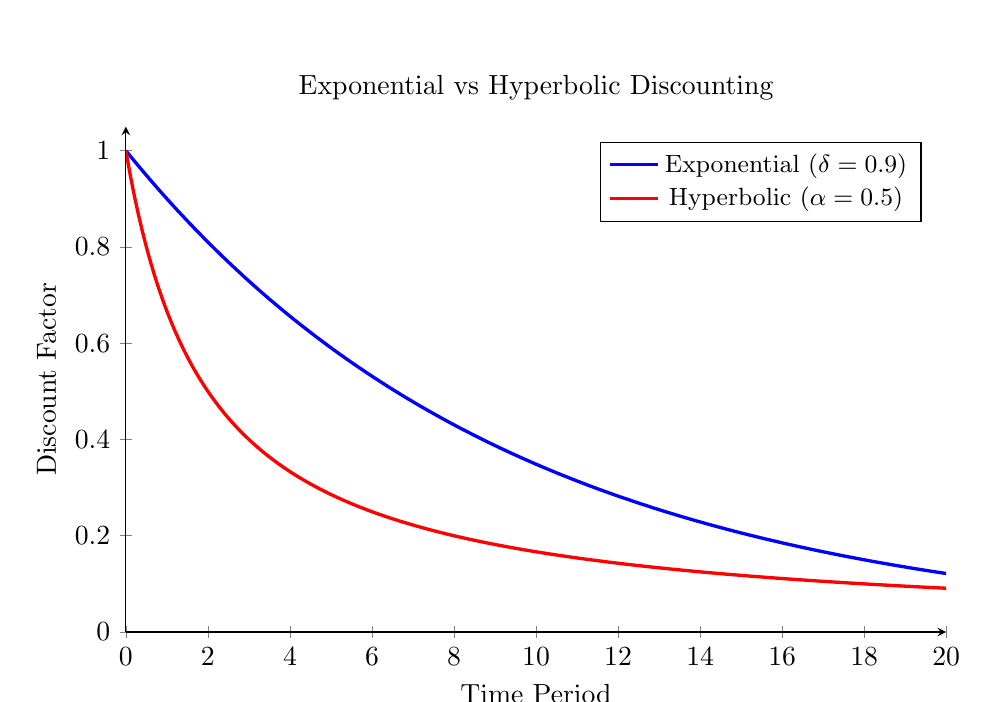
\begin{tikzpicture}

\begin{axis}[
    width=12cm,
    height=8cm,
    xlabel={Time Period},
    ylabel={Discount Factor},
    xmin=0, xmax=20,
    ymin=0, ymax=1.05,
    axis lines=left,
    title={Exponential vs Hyperbolic Discounting},
    legend style={at={(0.97,0.97)},anchor=north east,font=\small},
    samples=200
]

% Exponential discounting (BLUE)
\addplot[
    very thick,
    domain=0:20,
    color=blue
]
{0.9^x};

% Hyperbolic discounting (RED)
\addplot[
    very thick,
    domain=0:20,
    color=red
]
{1/(1+0.5*x)};

\legend{Exponential ($\delta=0.9$), Hyperbolic ($\alpha=0.5$)}

\end{axis}

\end{tikzpicture}

\caption{Comparison of exponential and hyperbolic discounting functions.}

\end{figure}

\begin{table}[H]
\centering
\small

\begin{tabularx}{\linewidth}{lX}
\toprule
 & Description \\
\midrule

\textbf{What the figure shows} 
& Two curves plotting the discount factor $D(t)$ against time $t$ from 0 to 20 periods. The exponential curve (e.g., $\delta^t$ with $\delta = 0.9$) declines smoothly and steeply --- roughly equal percentage decline in each period --- and reaches near-zero by period 20. The hyperbolic curve (e.g., $1/(1+0.5t)$) drops steeply from $t=0$ to $t=2$ but then flattens dramatically, approaching zero slowly and remaining above the exponential curve for large $t$. \\

\textbf{How to interpret it} 
& The steep initial drop in the hyperbolic curve is present bias: the agent dramatically undervalues even the near future relative to the present. But the flat tail means that for periods well in the future, the agent is relatively patient and approximately equally values different distant horizons. This generates the declining discount rate pattern. \\

\textbf{The critical feature} 
& The hyperbolic discounter overweights the present relative to all future periods, but does not especially distinguish between different future periods. This creates a systematic preference for the immediate option that emerges only when that option is immediate --- not when both options are still in the future. \\

\bottomrule
\end{tabularx}

\end{table}


\subsection{3.2 The Intuition for Time Inconsistency}


The hyperbolic discount function generates time inconsistency through a clear mechanism. Consider a person choosing between:
\begin{itemize}
\item \textbf{Option A:} A moderate reward at time $t=1$ (one week from now).
\item \textbf{Option B:} A larger reward at time $t=2$ (two weeks from now).
\end{itemize}

When evaluated from the present ($t=0$), both rewards are in the future. With $\alpha = 1$:
\begin{itemize}
\item $D(1) = 1/2$, $D(2) = 1/3$.
\item If Option B's reward is 60\% larger than Option A's, then $D(2) \times 1.6 = 0.533 > D(1) \times 1 = 0.5$. The agent \textbf{prefers Option B}.
\end{itemize}

Now one week passes. The agent is at $t=1$, and the choice is evaluated again:
\begin{itemize}
\item Option A is now immediate: $D(0) = 1$.
\item Option B is one week away: $D(1) = 1/2$.
\item Now $D(1) \times 1.6 = 0.8 < D(0) \times 1 = 1.0$. The agent \textbf{switches to Option A}.
\end{itemize}

The preference has \textit{reversed} --- not because any new information arrived, not because circumstances changed, but purely because one week has passed and the immediate option has become attractive in a way it was not when it was itself in the future. This is the essence of time inconsistency produced by hyperbolic discounting.

\textbf{The general principle:} Hyperbolic discounters prefer the patient option when both options are in the future but switch to the impatient option when the impatient choice becomes immediately available. They perpetually make plans to behave patiently in the future and perpetually break those plans when the future arrives.

\medskip


\section{4. The Quasi-Hyperbolic ($\beta$-$\delta$) Model}



\subsection{4.1 The Model}


The hyperbolic discount function $\frac{1}{1+\alpha t}$ captures the essential empirical patterns but is mathematically inconvenient---it does not have a recursive structure that makes dynamic optimisation tractable. For most economic analysis, a two-parameter approximation introduced by Laibson (1997) and building on earlier work by Phelps and Pollak (1968) is used instead.

The \textbf{quasi-hyperbolic} or \textbf{$\beta$-$\delta$ model} represents utility at time $t$ as:

$$U_t = u(c_t) + \beta \sum_{\tau=1}^{\infty} \delta^\tau \, u(c_{t+\tau})$$

where:
\begin{itemize}
\item $u(c_t)$ is the utility of immediate consumption (no discounting)
\item $\beta \in (0,1)$ is the \textbf{present bias parameter} --- an additional discount applied to all future periods uniformly
\item $\delta \in (0,1)$ is the standard long-run discount factor applied geometrically across future periods
\item When $\beta = 1$, the model reduces to standard exponential discounting
\end{itemize}

\textbf{Interpreting the parameters:}

The parameter $\beta$ represents the extra cost of \textit{any} delay --- the special additional discount that applies the moment a payoff moves from "now" into "the future." Once it is in the future, standard exponential discounting $\delta$ applies period by period. The key insight is that $\beta$ creates a \textit{discontinuity} between the present and all future periods, while $\delta$ governs patience \textit{within} the future.

\textbf{Calibrated values from the literature:}
\begin{itemize}
\item $\beta \approx 0.70$ to \$0.80\$ (reflecting the empirical finding that immediate gratification is discounted relative to even the very near future by 20--30\%)
\item $\delta \approx 0.95$ to \$0.99\$ (reflecting normal long-run patience consistent with standard discount rates of 1--5\% per year)
\end{itemize}


\subsection{4.2 How the Model Generates Present Bias}


Consider the discount weights the $\beta$-$\delta$ model assigns across periods for a person with $\beta = 0.7$ and $\delta = 0.97$:

\textbf{Table 4.3: Discount Weights in the $\beta$-$\delta$ Model ($\beta$ = 0.7, $\delta$ = 0.97)}


\begin{table}[H]
\centering
\small
\begin{tabularx}{\linewidth}{lYYY}
\toprule
Period & Exponential ($\delta^t$) & $\beta$-$\delta$ & Weight Drop \\
\midrule
t = 0 (now) & 1.000 & 1.000 & --- \\
t = 1 & 0.970 & 0.679 & \textbf{-32\%} \\
t = 2 & 0.941 & 0.659 & -3\% \\
t = 3 & 0.913 & 0.639 & -3\% \\
t = 4 & 0.885 & 0.620 & -3\% \\
t = 5 & 0.859 & 0.601 & -3\% \\
\bottomrule
\end{tabularx}
\end{table}


The dramatic feature is the \textbf{large drop from period 0 to period 1} (-32\%) followed by \textbf{small, steady drops in subsequent periods} (approximately -3\% per period thereafter). The agent is enormously impatient about the transition from now to tomorrow but approximately equally patient between any two future periods. This captures the "steep initial drop, flat tail" of the hyperbolic discount function in a tractable two-parameter form.

\textbf{Figure 4.2: Comparing Exponential and $\beta$-$\delta$ Discount Weights}

\begin{figure}[ht]
\centering

\begin{tikzpicture}
\begin{axis}[
    width=\textwidth,
    height=0.55\textheight,
    xlabel={Period},
    ylabel={Discount Weight},
    xmin=0, xmax=7,
    ymin=0.5, ymax=1.05,
    axis lines=left,
    title={$\beta$-$\delta$ vs Exponential Discounting ($\beta=0.7$, $\delta=0.97$)},
    legend style={
        at={(0.98,0.98)},
        anchor=north east,
        font=\small
    },
    tick label style={font=\small},
    label style={font=\small}
]

% Exponential discounting
\addplot[
    blue,
    thick,
    mark=square*
] coordinates {
    (0,1)
    (1,0.97)
    (2,0.9409)
    (3,0.9127)
    (4,0.8853)
    (5,0.8587)
    (6,0.8330)
    (7,0.8080)
};

% Beta-delta model
\addplot[
    red,
    thick,
    mark=*
] coordinates {
    (0,1)
    (1,0.7)
    (2,0.679)
    (3,0.659)
    (4,0.639)
    (5,0.620)
    (6,0.601)
    (7,0.583)
};

% Present bias annotation
\draw[<->, thick]
(axis cs:1,0.97) -- (axis cs:1,0.7)
node[midway,right, font=\scriptsize, align=left]
{$\beta = 0.7$\\present bias drop};

\legend{
    Exponential ($\delta=0.97$),
    $\beta$-$\delta$ ($\beta=0.7$, $\delta=0.97$)
}

\end{axis}
\end{tikzpicture}

\caption{Comparison of exponential and quasi-hyperbolic discounting.}
\end{figure}


\begin{table}[H]
\centering
\small
\begin{tabularx}{\linewidth}{lY}
\toprule
 & Description \\
\midrule
\textbf{What the figure shows} & Two step-function graphs plotting discount weights at periods 0 through 7. The exponential weights decline smoothly from 1.000 to 0.808. The $\beta$-$\delta$ weights show a sharp drop from 1.000 at $t=0$ to 0.679 at $t=1$, then decline gradually in parallel with the exponential curve but at a uniformly lower level. A bracket labels the gap between the two curves at $t=1$ as the "present bias drop" caused by $\beta = 0.7$. \\
\textbf{How to interpret it} & The gap between the two curves at $t=1$ is entirely attributable to $\beta$. From period 1 onward, both curves decline at the same rate (determined by $\delta$), maintaining a constant vertical gap. The $\beta$-$\delta$ model essentially "handicaps" all future periods equally, making them 30\% less valuable than they would be without present bias. \\
\bottomrule
\end{tabularx}
\end{table}



\subsection{4.3 Time Inconsistency in the $\beta$-$\delta$ Model}


The $\beta$-$\delta$ model generates time inconsistency through the same mechanism as the hyperbolic model. A formal illustration:

\textbf{The Preference Reversal.} Suppose an agent is choosing between:
\begin{itemize}
\item \textbf{Option A:} Receive utility $u_A$ at time $t = 1$.
\item \textbf{Option B:} Receive utility $u_B > u_A$ at time $t = 2$.
\end{itemize}

\textbf{At time 0 (future perspective):} $$U_0(A) = \beta \delta^1 u_A = \beta \delta u_A$$ $$U_0(B) = \beta \delta^2 u_B$$

Agent prefers B if $u_B > u_A / \delta$ --- the standard patience condition with $\delta$ but not involving $\beta$, because $\beta$ appears in both terms and cancels.

\textbf{At time 1 (A is now immediate):} $$U_1(A) = u_A \quad \text{(no discounting --- A is immediate)}$$ $$U_1(B) = \beta \delta^1 u_B \quad \text{(B is now one period away)}$$

Agent prefers B if $u_B > u_A / (\beta \delta)$.

Since $\beta < 1$, the threshold $u_A / (\beta \delta) > u_A / \delta$. So the agent who preferred B at time 0 may now prefer A at time 1 --- the preference has reversed. Specifically, if:

$$\frac{u_A}{\delta} < u_B < \frac{u_A}{\beta \delta}$$

then the agent prefers B at time 0 but A at time 1. This is the \textbf{preference reversal} --- the mathematical signature of time inconsistency.

\medskip


\section{5. Procrastination}



\subsection{5.1 The Economics of Procrastination}


Present bias does not merely affect consumption and savings decisions. It generates one of the most pervasive phenomena in daily life: \textbf{procrastination} --- the systematic delay of effortful actions even when the agent genuinely wants to complete them and even when delay is costly.

O'Donoghue and Rabin (1999, 2001) provided the formal economic analysis. Consider an agent who must complete a task at some point over a horizon of $T$ periods. The task involves an effort cost $c$ (experienced in the period when it is done) and generates a benefit $b$ (received at the end of the horizon, regardless of when the task is completed). A rational patient agent (with $\beta = 1$) would complete the task in the first period --- the cost is the same whenever incurred, so there is no point in delaying.

A present-biased agent ($\beta < 1$) behaves differently. In period $t$, completing the task now costs $c$ immediately (no discounting), while waiting means the cost is $c$ in period $t+1$ --- but as seen from today, that future cost is discounted by $\beta\delta$. So the agent compares:

\begin{itemize}
\item \textbf{Do it now:} cost of $c$ borne immediately.
\item \textbf{Wait one period:} discounted cost of $\beta \delta c$ borne next period.
\end{itemize}

As long as $\beta \delta c < c$ --- which holds whenever $\beta \delta < 1$, i.e., practically always --- the agent prefers to wait. But crucially, \textit{the same logic applies in every period}. The agent arrives at period $t+1$ and again prefers to wait --- because now the cost of waiting is again discounted by $\beta\delta$, making waiting again preferable to acting. The agent perpetually finds it rational to defer the task one more period.

\textbf{The procrastination trap:} With sufficient present bias, the agent delays in every period until a deadline forces action. If no deadline exists, the task may never be completed. This is a pure consequence of time-inconsistent preferences --- not laziness, not disorganisation, not insufficient commitment to the goal.


\subsection{5.2 An Illustration: The Essay Problem}


Consider a student with a take-home essay due at the end of a 6-week term. The essay takes 3 hours. The student is asked to make their plan at the start of term:

\begin{itemize}
\item \textbf{At start of term (6 weeks before the deadline):} Writing the essay this week has a cost of 3 hours now; writing it next week has a cost of 3 hours next week, discounted by $\beta\delta$. Even a mildly present-biased student prefers to wait.
\item \textbf{One week later:} The same logic applies. Wait again.
\item \textbf{Two weeks later, three weeks later, four weeks later...} Same logic. Same decision.
\item \textbf{Night before deadline:} Now there is no future period to defer to. The student writes the essay in a panic.
\end{itemize}

The student's experience is:
\begin{itemize}
\item Each week: "I'll write it next week."
\item At the end: genuine surprise and distress that they did not write it earlier.
\end{itemize}

This pattern --- sincere intention to act in the future, perpetual deferral when the future arrives --- is the hallmark of naive present bias. The student was not lying when they planned to write the essay in week 1. Their plan was sincere. But their preferences changed when week 1 arrived.

\begin{researchbox}
\textbf{Research Study: Procrastination, Deadlines, and Performance}\\[4pt]

\textbf{Researchers:} Dan Ariely and Klaus Wertenbroch\\[4pt]
\textbf{Year:} 2002\\[4pt]
\textbf{Research Question:} Do self-imposed deadlines improve performance relative to free choice of submission timing, even when there is no external requirement?\\[4pt]
\textbf{Method:} Students in two sections of an MIT executive education programme were assigned three papers over the term. One group received evenly spaced, instructor-imposed deadlines. The other group was allowed to set their own deadlines, with the only requirement being that all three papers be submitted by the end of the term. A third condition (end-of-term deadline) was also used in a related study.\\[4pt]
\textbf{Results:} Students who received imposed deadlines earned the best grades. Students who chose their own deadlines earned the second-best grades --- and notably, most students chose to space their deadlines relatively evenly, demonstrating some awareness of their procrastination tendency. Students with a single end-of-term deadline earned the worst grades.\\[4pt]
\textbf{Economic Interpretation:} The ability to choose deadlines --- even without binding constraints --- improved performance relative to unconstrained choice, suggesting that students are at least partially sophisticated about their own present bias and attempt to create commitment through self-imposed milestones. The gap between imposed and self-imposed deadlines shows that even partial sophistication is insufficient to fully overcome procrastination.\\[4pt]
\textbf{Behavioural Insight:} Deadlines work because they remove the option to delay. Present-biased agents systematically underestimate the cost of future delay and overestimate their future resolve. External structures that constrain future choices --- imposed deadlines, scheduled appointments, automatic reminders --- substitute for the self-control the agent lacks.\\[4pt]
\end{researchbox}

\textbf{Canadian Evidence.} A study at the University of British Columbia found that providing students with digital calendar reminders for major assessment deadlines, along with suggested milestone schedules, improved grade point averages by an average of 0.4 points relative to a control group that received no such structure. This modest intervention --- which imposed no costs and required no change in course content --- reduced procrastination through a combination of salience (making the deadline more cognitively available) and mild commitment.

\medskip


\section{6. Naïve versus Sophisticated Agents}



\subsection{6.1 The Distinction}


Not all present-biased agents are alike. A crucial dimension of variation concerns \textbf{self-knowledge}: does the agent understand that they are present-biased?

O'Donoghue and Rabin (2001) formalised this distinction by distinguishing between:

\textbf{Naïve agents} believe their future self will behave exactly as their current self plans. They perceive their present-bias parameter as $\hat{\beta} = 1$ --- they mistakenly believe they have no present bias and will faithfully execute all plans made today. Each period, they make a plan they fully intend to follow. Each period, when it arrives, present bias causes them to deviate. They are perpetually surprised by their own behaviour and perpetually optimistic about future behaviour.

\textbf{Sophisticated agents} correctly understand that their future self has present bias. They perceive their present-bias parameter accurately: $\hat{\beta} = \beta < 1$. They know that when a temptation arrives, their future self will yield to it. This self-awareness allows them to take \textbf{preemptive action} --- to constrain or influence their future self's choices before the temptation arrives.

\textbf{Table 4.4: Comparing Naïve and Sophisticated Present-Biased Agents}


\begin{table}[H]
\centering
\small
\begin{tabularx}{\linewidth}{lYY}
\toprule
Feature & Naïve Agent & Sophisticated Agent \\
\midrule
Self-knowledge of present bias & None ($\hat{\beta} = 1$) & Accurate ($\hat{\beta} = \beta < 1$) \\
Plans for the future & Sincere but overoptimistic & Accurately pessimistic about future behaviour \\
Response when temptation arrives & Gives in; surprised & Gives in; not surprised --- anticipated this \\
Use of commitment devices & None --- sees no need & Actively seeks commitment devices \\
Pattern of behaviour & Perpetual fresh starts, repeated failures & More strategic; avoids placing self in tempting situations \\
Famous archetype & Every New Year's resolution & Ulysses and the Sirens \\
\bottomrule
\end{tabularx}
\end{table}


Between these extremes lies the empirically important case of \textbf{partial sophistication}: agents who recognise they have some present bias but underestimate its magnitude. They attempt to pre-commit and to create structure for their future selves, but their strategies are insufficiently powerful to fully overcome the bias. The students in Ariely and Wertenbroch's experiment who chose to space deadlines but not evenly enough exemplify this: partial sophistication led to partial improvement but not full correction.


\subsection{6.2 Ulysses and the Sirens}


The mythological story of Ulysses and the Sirens is perhaps the most vivid illustration of sophisticated present-bias management in all of literature.

In Homer's \textit{Odyssey}, Ulysses is warned that his ship will sail past the island of the Sirens, whose song is so irresistible that every sailor who hears it leaps overboard in an attempt to swim to them. Ulysses wishes to hear the Sirens' song --- a unique experience --- but knows that his future self, once within earshot, will be unable to resist throwing himself overboard. The sophisticated solution: before reaching the Sirens, Ulysses orders his crew to tie him to the mast and to ignore any commands he gives to be released until the ship has passed. He additionally orders the crew to plug their own ears with beeswax so they cannot hear the song themselves.

This is a textbook commitment device. Ulysses, at time 0, correctly anticipates that his time-1 self will have radically different preferences (the Siren-influenced self will desperately want to be freed). He uses his authority \textit{now}, before the temptation arrives, to bind his future self in a way his future self cannot undo. The binding is credible precisely because the crew cannot hear his future pleas.

The economic structure is:
\begin{itemize}
\item \textbf{Time 0:} Ulysses is rational, far-sighted, sophisticated.
\item \textbf{Time 1:} Ulysses is present-biased, overwhelmed by immediate temptation.
\item \textbf{Commitment device:} Removes future-self's ability to act on time-1 preferences.
\end{itemize}

The story is so resonant because it describes a genuinely common human predicament: we frequently prefer, in our calm, far-sighted moments, to constrain the choices of our impulsive future selves. The Ulysses contract is a commitment to future constraint enacted before the impulse arrives.


\subsection{6.3 The Dangers of Naivety}


Naïve agents can behave very poorly relative to their own long-run interests --- not because they want to, but because they persistently underestimate how strongly their future self will be pulled toward the immediate option.

Consider the following consequence. A naïve present-biased agent and a sophisticated present-biased agent both face the same long-term task. The sophisticated agent, knowing they will procrastinate if left unconstrained, immediately signs up for a structured programme with binding deadlines. The naïve agent, believing they will act on their good intentions, does not sign up for any structure. When the deadline approaches, the naïve agent finds themselves in the same position as always --- acting at the last moment or not at all, genuinely baffled by their own behaviour.

O'Donoghue and Rabin (2001) showed formally that naïve agents can cycle through identical failed attempts indefinitely, making the same plan and experiencing the same failure in every period. They called this the \textbf{naïve perpetual procrastination trap}: the agent always means to act this time and always finds that future-self fails them, yet because each failure is unexpected, no systemic corrective action is taken.

This has policy implications. Interventions designed to help present-biased agents are most effective when targeted at:
\begin{itemize}
\item Naïve agents who would benefit from information about their own procrastination tendency.
\item Both naive and sophisticated agents through structural changes (defaults, automatic enrolment) that work independently of self-knowledge.
\end{itemize}

\medskip


\section{7. Commitment Devices}



\subsection{7.1 Definition and Logic}


A \textbf{commitment device} is a mechanism that a sophisticated present-biased agent uses in advance to constrain their future self's choices, remove temptations, or impose costs on future behaviour they anticipate wanting to avoid. The defining features are:

\begin{enumerate}
\item \textbf{Precommitment:} The device is activated at time 0, before the temptation arrives at time 1.
\item \textbf{Binding constraint:} The device genuinely limits what the future self can do --- it is not merely a resolution or intention.
\item \textbf{Credibility:} The future self cannot easily circumvent the device.
\end{enumerate}

The economic logic is subtle. A commitment device is voluntarily adopted by the present self precisely to restrict the options of the future self. From a standard rational-choice perspective, restricting your own options can never be beneficial --- more options are weakly better. But for a present-biased agent, the future self's preferences are, in the anticipation of the present self, suboptimal. The present self genuinely prefers to prevent the future self from indulging the bias --- and is willing to pay a cost (in the form of reduced flexibility) to achieve this.


\subsection{7.2 Historical and Modern Examples}


\textbf{Ulysses contracts.} As described above: pre-binding oneself to a course of action before the temptation arrives. Named after the Odyssey example, Ulysses contracts have been formalised in several legal and medical contexts. Psychiatric advance directives --- in which a person specifies in advance what medical treatment they want during a future episode of psychosis, before they lose the capacity for rational decision --- are a legally recognised form of Ulysses contract in several countries, including Canada.

\textbf{Christmas clubs.} A Christmas club is a low-interest bank savings account (or, historically, a scheme organised through an employer or union) to which a person makes regular contributions throughout the year, with the funds inaccessible until December. The device commits the present self to save, by making early withdrawal costly or impossible, precisely because the saver knows their future self will otherwise spend the money. Christmas clubs were extremely popular in the United States and Canada in the mid-twentieth century, at a time when most other savings vehicles were accessible on demand. Their appeal was not the interest rate --- it was the commitment.

\textbf{Layaway plans.} A retail arrangement in which a consumer makes a deposit on a product and pays in instalments before taking possession. From a standard economic perspective, layaway is dominated by a credit card purchase (you get the product now, rather than later). But for a present-biased consumer who fears they will spend the money on something else if they have it in hand, layaway commits them to the planned purchase --- the money is gone (in the hands of the retailer) before temptation can intervene.

\textbf{Commitment savings accounts.} Modern financial innovation has produced commitment savings products that make savings withdrawals costly or impossible before a target date or target amount is reached. These products are particularly interesting because they attract sign-ups from people who understand their present bias and are willing to accept a lower return in exchange for a binding commitment.

\begin{researchbox}
\textbf{Research Study: Commitment Savings in the Philippines --- Tying Odysseus to the Mast}\\[4pt]

\textbf{Researchers:} Nava Ashraf, Dean Karlan, and Wesley Yin\\[4pt]
\textbf{Year:} 2006\\[4pt]
\textbf{Research Question:} Do commitment savings accounts --- which lock funds until a target date or amount is reached --- increase savings among present-biased agents?\\[4pt]
\textbf{Method:} A rural bank in the Philippines was assisted in developing a new commitment savings product called "SEED" (Save, Earn, Enjoy Deposits). SEED accounts did not offer a higher interest rate than standard accounts --- the only difference was that they were locked until the account holder reached a self-chosen target date or target amount. The product was randomly offered to a sample of existing customers. A control group received no offer.\\[4pt]
\textbf{Results:} After 12 months, account holders in the SEED group had savings balances 82\% higher than those in the control group. Take-up of the product was only 28\% --- but among those who took it up, the effect was very large.\\[4pt]
\textbf{Economic Interpretation:} The 82\% savings increase --- achieved with no financial incentive beyond the commitment structure --- is among the largest effects ever recorded from a savings intervention. The modest take-up (28\%) is consistent with a mix of naive and sophisticated agents: sophisticated agents recognise the value of committing and sign up; naive agents see no need. The large effect among adopters confirms that the commitment mechanism, not selection, drives savings.\\[4pt]
\textbf{Behavioural Insight:} The SEED study demonstrates that people are willing to pay for commitment --- they accept account restrictions with no interest premium because the binding constraint is itself valuable. This overturns the standard economic prediction that agents never benefit from having fewer options.\\[4pt]
\end{researchbox}

\textbf{stickK.com.} A modern online platform founded by Yale economists Dean Karlan and Ian Ayres that institutionalises the commitment contract. Users specify a goal (e.g., exercise three times per week), a stake (money they pledge to lose if they fail), and a referee (who verifies compliance). If the goal is not met, the money is forfeit --- either to a charity of the user's choice or, for maximum pain, to an organisation they actively dislike. The site reports active stakes of approximately \$700,000 per day. The anti-charity option is particularly interesting: it exploits loss aversion (losing money is painful) combined with the additional sting of that money going to a disliked cause. The empirical evidence on stickK-style commitment contracts (Karlan et al., 2016) finds modest but statistically reliable improvement in goal achievement.

\textbf{Automatic savings transfers.} Modern banking technology has made one of the most powerful commitment devices available to virtually everyone: automatic regular transfers from a chequing account to a savings account, scheduled at the moment of a paycheck deposit. Services like Simplii Financial and Tangerine in Canada allow users to set up automatic transfers that remove money from the accessible chequing account before spending temptation can operate on it. The mechanism is not perfectly binding (transfers can be cancelled), but the friction of cancellation --- requiring a deliberate action --- is sufficient to reduce present-bias-driven raiding of savings.


\subsection{7.3 Evaluating Commitment Devices}


A well-designed commitment device has three key properties:
\begin{enumerate}
\item \textbf{It pre-commits.} The device is set up before the temptation arrives. If the agent can cancel the commitment the moment temptation appears, it provides no protection.
\item \textbf{It is binding.} The commitment imposes a genuine cost on deviation --- whether financial, reputational, or practical.
\item \textbf{The future self cannot easily circumvent it.} The more easily the future self can undo the commitment, the weaker the protection.
\end{enumerate}

Not all commitment devices achieve all three. A resolution ("I resolve to exercise more") fails on all three counts: it requires no action beyond declaring intent, it imposes no cost on deviation, and the future self faces no barrier to breaking it. A pre-paid gym membership scores better but is easily circumvented by simply not going. An automatic payroll deduction to a locked retirement account scores highest: the money is removed before spending temptation arises, and accessing it before retirement involves penalties that constitute genuine costs.

\medskip


\section{8. Savings Behaviour and the Canadian Undersaving Puzzle}



\subsection{8.1 The Life-Cycle Model and Its Prediction}


The standard model of household savings is the \textbf{life-cycle hypothesis} (Modigliani and Brumberg, 1954; Friedman, 1957). A rational, time-consistent agent solves a lifetime optimisation problem: in working years, earn income and save; in retirement, spend down savings. The agent smooths consumption across the lifecycle, saving enough in working years to maintain living standards in retirement.

Under this model, households should build up substantial savings during their working years and draw them down in retirement. The model makes specific predictions about the savings rate: it should be roughly constant and positive during working years, with some variation depending on age, income, and expected retirement date.

The Canadian evidence is difficult to reconcile with this prediction:
\begin{itemize}
\item The Canadian household savings rate fell from over 20\% in 1982 to 2.5\% in 2005 before recovering partially after the 2008 financial crisis.
\item As of 2024, the savings rate sits at approximately 5--6\% --- well below what most financial planners consider adequate for retirement security.
\item A 2023 BMO survey found that 41\% of Canadians have \textit{no} retirement savings at all.
\item Only 27\% of eligible Canadians contributed to their RRSPs in 2022, leaving average unused contribution room of over \$25,000 per filer.
\item 47\% of Canadians report living paycheque to paycheque (FP Canada, 2023).
\end{itemize}

These patterns cannot be explained by poverty alone --- they persist among middle-income households, where the life-cycle model predicts comfortable savings rates. Nor can they be explained by information deficits: 93\% of Canadians know what an RRSP is. The problem is not that people don't know saving is important. It is that the present self continually makes spending decisions that the future self will regret.

\textbf{Figure 4.3: Canadian Household Savings Rate, 1982--2024}

\begin{figure}[h!]
\centering
\begin{tikzpicture}
\begin{axis}[
    width=0.95\textwidth,
    height=0.6\textheight,
    axis lines=left,
    xlabel={\small Year},
    ylabel={\small Savings Rate (\%)},    
    xmin=1980, xmax=2025,
    ymin=0, ymax=32,
    xtick={1980,1985,1990,1995,2000,2005,2010,2015,2020,2025},
    ytick={0,5,10,15,20,25,30},
    tick label style={font=\small},
    label style={font=\small},
    title style={font=\small},
    title={Canadian Household Savings Rate},
    grid=both,
    grid style={dotted,gray!30},
    clip=false,
]

% Main series
\addplot[
    very thick,
    blue
] coordinates {
  (1982,20.2)
  (1985,17)
  (1990,13)
  (1995,9)
  (2000,5.3)
  (2005,2.5)
  (2008,5)
  (2010,6)
  (2015,4)
  (2019,3.5)
  (2020,12)
  (2021,28)
  (2022,7)
  (2024,5.3)
};

% Horizontal target line
\draw[dashed, teal, thick]
    (axis cs:1980,10) -- (axis cs:2025,10)
    node[pos=1.02, above, font=\small, text=teal] {10\% target};

\end{axis}
\end{tikzpicture}
\end{figure}


\begin{table}[H]
\centering
\small
\begin{tabularx}{\linewidth}{lY}
\toprule
 & Description \\
\midrule
\textbf{What the figure shows} & A time-series graph of the Canadian household savings rate from 1982 to 2024. A near-horizontal teal dashed line at 10\% represents the approximate savings rate consistent with adequate retirement preparation. The actual data line starts high (above 20\% in 1982), then declines steeply through the 1990s and early 2000s, reaching a low of 2.5\% in 2005. It partially recovers after 2008, then spikes dramatically in 2020 and 2021 (12--28\%) during the COVID-19 pandemic when forced savings occurred, before falling back toward 5--6\% in 2022--2024. \\
\textbf{How to interpret it} & The long-term decline in the savings rate, from a level adequate for life-cycle smoothing to one that will leave many households with inadequate retirement income, is consistent with increasing present bias effects in an environment of rising consumer credit availability, expanding advertising, and growing temptation through consumption options. The COVID spike --- a forced experiment in reduced consumption opportunity --- demonstrates that the savings capacity exists; the issue is present-bias-driven spending when consumption opportunities are available. \\
\bottomrule
\end{tabularx}
\end{table}



\subsection{8.2 Present Bias as the Mechanism}


The $\beta$-$\delta$ model provides a precise explanation. A household with $\beta = 0.7$ and $\delta = 0.97$ values retirement income roughly 30\% less than exponential discounting would predict, all else equal. Even more consequentially, the model predicts that the household's \textit{intention} to save will persistently exceed its \textit{actual} saving --- because planning is done when retirement is far away (and both the current self's plan and the future self's action are discounted symmetrically), but the decision not to save is made when current consumption is immediate.

Laibson, Repetto, and Tobacman (2001) estimated that present bias ($\beta < 1$) explained approximately 75\% of credit card debt among US households who simultaneously held substantial savings in illiquid assets. These households were in effect paying 19\% interest on credit card debt while earning 4--6\% on savings --- a gap that persists not because of ignorance of arithmetic but because the present self continuously finds reasons to spend now rather than pay down debt.

An important implication: \textbf{the problem is structural, not informational}. Financial education that tells people "you should save more" addresses a problem that people already know about. What is needed is structural change --- making saving the default, removing friction from saving while adding friction to spending --- that works with present-biased preferences rather than against them.

\medskip


\section{9. Save More Tomorrow}


\begin{researchbox}
\textbf{Research Study: Save More Tomorrow (SMarT)}\\[4pt]

\textbf{Researchers:} Richard Thaler and Shlomo Benartzi\\[4pt]
\textbf{Year:} 2004\\[4pt]
\textbf{Research Question:} Can a pre-commitment savings programme increase contribution rates among employees who want to save more but fail to do so?\\[4pt]
\textbf{Method:} Thaler and Benartzi developed the SMarT programme in partnership with a mid-sized US manufacturing company. The programme offered employees a pre-commitment: agree \textit{now} to increase your retirement savings contribution by a fixed amount with \textit{each future pay raise}. Employees did not experience an immediate reduction in take-home pay (because the increase was timed with a raise), and contributions were increased automatically without requiring any future action. A financial planner met with employees to discuss savings goals; those who agreed they were undersaving were offered the SMarT commitment.\\[4pt]
\textbf{Results:} Among employees who used the SMarT programme:\\[4pt]
- Savings rate rose from 3.5\% at baseline to 6.5\% after the first raise, 9.4\% after the second, and 11.6\% after the third.
- Participation rate in the company pension plan rose from 3.5\% to 13.6\% over the same period.
- The control group (employees offered standard financial advice) showed essentially no change: savings rates remained at approximately 3.5--3.8\% throughout.

\textbf{Economic Interpretation:} Three features of the SMarT design combat present bias directly:\\[4pt]
1. \textbf{Pre-commitment:} Employees agreed to future savings increases \textit{before} the raise arrived --- when both the cost and benefit were in the future. At this point, present bias does not distort the comparison.
2. \textbf{Raise-synchronisation:} By increasing savings at the moment of a pay raise, the employee never experiences a reduction in take-home pay relative to their prior reference point. Loss aversion is avoided.
3. \textbf{Automaticity:} Increases happen without requiring any future action. Inertia --- which normally causes present-biased agents to remain at low savings rates --- is now working in favour of higher savings.

\textbf{Policy Legacy:} The SMarT design was incorporated into the US Pension Protection Act of 2006, which encouraged automatic enrolment and automatic escalation in employer-sponsored retirement plans. In Canada, WorkSafeBC adopted an automatic escalation provision in its pension plan design in 2018, consistent with SMarT principles.\\[4pt]
\end{researchbox}
\newpage
\textbf{Figure 4.4: SMarT Programme Results}

\begin{figure}[htbp]
\centering

\begin{tikzpicture}
\begin{axis}[
    width=0.85\textwidth,
    height=0.55\textheight,
    ybar,
    bar width=0.35cm,
    enlarge x limits=0.25,
    ylabel={Savings Rate (\%)},
    symbolic x coords={Baseline,Year 1,Year 2,Year 3},
    xtick=data,
    ymin=0,
    ymax=14,
    ytick={0,2,4,6,8,10,12,14},
    nodes near coords,
    nodes near coords style={
        font=\small,
        /pgf/number format/fixed,
        /pgf/number format/precision=1
    },
    title={SMarT Program Results},
    title style={font=\bfseries},
    legend style={
        at={(0.5,-0.18)},
        anchor=north,
        legend columns=2,
        font=\small
    },
    axis lines=left,
    tick label style={font=\small},
    label style={font=\small},
    grid=major,
    grid style={dashed,gray!30}
]

% SMarT group
\addplot[
    fill=teal!60,
    draw=teal!80
]
coordinates{
    (Baseline,3.5)
    (Year 1,6.5)
    (Year 2,9.4)
    (Year 3,11.6)
};

% Control group
\addplot[
    fill=orange!60,
    draw=orange!80
]
coordinates{
    (Baseline,3.5)
    (Year 1,3.6)
    (Year 2,3.7)
    (Year 3,3.8)
};

\legend{
    SMarT group,
    Control group
}

\end{axis}
\end{tikzpicture}

\caption{Savings rates increased substantially among participants in the SMarT program relative to the control group.}
\end{figure}


\begin{table}[H]
\centering
\small
\begin{tabularx}{\linewidth}{lY}
\toprule
 & Description \\
\midrule
\textbf{What the figure shows} & A grouped bar chart showing savings rates at baseline and in each of three years for the SMarT group and the control group. The SMarT bars rise from 3.5\% to 11.6\% across the three-year period. The control bars remain approximately flat at 3.5--3.8\%. \\
\textbf{How to interpret it} & The 8.1 percentage point increase in savings rate --- from 3.5\% to 11.6\% --- achieved without any financial incentive (no employer match, no tax credit) demonstrates the power of pre-commitment and automaticity in overcoming present bias. The flat control line shows that standard financial advice, which addresses the wrong problem (information rather than inertia and present bias), is ineffective. \\
\bottomrule
\end{tabularx}
\end{table}


The SMarT programme's success illustrates a general principle that runs through this textbook: the most effective interventions for present-biased agents are those that \textbf{remove the moment of decision} from the point of temptation. When the decision to save is made months in advance (before the raise), present bias does not operate. When it must be made each month at the moment of receiving one's paycheque, present bias systematically wins.

\medskip


\section{10. Addiction and Present Bias}



\subsection{10.1 Addictive Goods and Intertemporal Bias}


The present-bias framework illuminates one of the most economically and socially significant forms of self-control failure: addiction. Addictive goods --- tobacco, alcohol, gambling, certain foods, social media --- share a common intertemporal structure: the pleasures they provide are immediate, while their costs (health consequences, financial harm, relationship damage) are delayed. Present bias therefore causes systematic over-consumption of addictive goods relative to what the agent would choose from a long-run perspective.

Consider a smoker. At any given moment, the decision to smoke a cigarette involves:
\begin{itemize}
\item \textbf{Immediate benefit:} The pleasure and craving relief of nicotine.
\item \textbf{Delayed cost:} A marginal increase in risk of lung cancer, heart disease, and other conditions, materialising over decades.
\end{itemize}

A time-consistent agent would trade off these correctly, arriving at a long-run optimal level of consumption. A present-biased agent ($\beta < 1$) systematically underweights the future costs relative to the present pleasure. The optimal quantity from a long-run perspective is lower than what is actually consumed.


\subsection{10.2 Canadian Smoking Data}


Canadian smoking statistics illustrate both the problem and the partial success of policy interventions designed to address it:
\begin{itemize}
\item The Canadian smoking rate has fallen from approximately 50\% in 1966 to approximately 13\% in 2019 --- a remarkable public health achievement, driven in part by information campaigns, warning labels, and taxation.
\item Despite this progress, approximately \textbf{70\% of current smokers report wanting to quit}, and roughly \textbf{50\% attempt to quit in any given year}.
\item Among unassisted quit attempts, the six-month success rate is approximately \textbf{5\%}.
\item British Columbia's QuitNow programme --- which provides counselling, medication assistance, and structured support --- achieves a \textbf{23\% six-month quit rate}, nearly five times the unassisted rate.
\end{itemize}

The gap between the 70\% who want to quit and the 5\% who succeed without help is a direct measure of the self-control problem that present bias creates. These are not people who have decided smoking is worth its health consequences --- they have explicitly decided they want to stop. The failure to follow through is the present-bias failure in action.

The classical pattern of the naive present-biased smoker: "I'll quit on Monday." Arrives on Monday: "I'll quit next Monday." This cycle, repeated across months and years, characterises the experience of a large fraction of current smokers.


\subsection{10.3 Policy: Corrective Taxation and Present Bias}


The conventional economic justification for taxing cigarettes is as a \textbf{Pigouvian tax}: correcting for the external costs that smoking imposes on others (secondhand smoke, healthcare costs borne by the public). But O'Donoghue and Rabin (2006) showed that present bias provides an additional and distinct justification: even when there are no external costs, a corrective tax is optimal if consumers are present-biased and naive.

\textbf{The argument:} A present-biased naive agent over-consumes addictive goods relative to their own long-run preferences --- the preferences they would express if making a careful, distant decision about how much they want to consume over their lifetime. The over-consumption is not a case of preferences that the policymaker should simply accept; it is a case of revealed present-biased preferences that diverge from the agent's own long-run welfare.

A tax that raises the price of the addictive good reduces consumption toward the agent's long-run optimum. Because the tax is paid in the present (where present-biased agents weight it fully), while the health costs it helps avoid are in the future (where present-biased agents underweight them), the tax can correct the intertemporal distortion. Formally, the optimal corrective tax equals the marginal internalised damage --- the present value of the health costs that the present-biased agent fails to internalise due to their bias.

\textbf{The caveat for sophisticated agents:} If all agents are sophisticated --- they fully understand their present bias and have correctly modelled its consequences --- then they have already incorporated their self-control problems into their consumption decisions, and a corrective tax may impose costs without benefits (sophisticated agents are already optimising given their preferences). In practice, the optimal tax depends on the mix of naive and sophisticated agents in the population, and on the extent to which commitment devices are available as substitutes.

The policy implications:
\begin{enumerate}
\item \textbf{For naive agents:} Higher taxes are justified to correct present-bias-driven over-consumption.
\item \textbf{For sophisticated agents:} Commitment devices (nicotine patches, prescription programmes, QuitNow-style counselling) are more efficient than taxes, which reduce consumption but also impose deadweight costs on agents who are already managing their bias.
\item \textbf{For a mixed population:} The optimal policy typically involves both taxation (to protect naive agents) and commitment facilitation (to help sophisticated agents).
\end{enumerate}

\medskip


\section{11. Policy Implications: From Theory to Intervention}


The theory of present bias and time inconsistency generates a rich set of policy implications. The common thread is that effective policy for present-biased agents must work with intertemporal preference structure --- targeting decisions at the time when present bias is not operative (when the temptation is distant) and using automaticity to avoid placing the decision at the moment of temptation.


\subsection{11.1 Defaults and Automatic Enrolment}


Madrian and Shea (2001) documented that switching a workplace retirement savings plan from opt-in (employees must actively choose to enrol) to automatic enrolment (employees are enrolled by default but can opt out) increased participation rates from approximately 49\% to 86\%. The plan and the financial incentives were identical --- the only change was which action was required to achieve enrolment.

The mechanism: automatic enrolment exploits \textbf{status quo bias} and \textbf{inertia} --- both related to present bias --- on behalf of the saver. The default state now involves saving; doing nothing (the path of least resistance for a present-biased agent) results in saving rather than not saving. Crucially, the programme does not restrict anyone's freedom to opt out --- it merely changes which choice requires action.

This intervention is studied in depth in Chapter 5 (Savings Behaviour) and Chapter 9 (Nudges and Choice Architecture), where its design, effectiveness, and limits are examined in detail.


\subsection{11.2 Mandatory Savings Systems}


A more aggressive intervention is \textbf{mandatory savings} --- removing the choice entirely. Australia's Superannuation system, introduced in 1992, requires employers to contribute 11\% of wages into a private retirement savings fund on behalf of each employee. The employee cannot access these funds before retirement age except in narrow hardship circumstances.

This policy is explicitly designed to override present-bias-driven undersaving. Its effectiveness is documented: Australian workers have substantially higher retirement savings than comparable workers in countries with voluntary systems. The trade-off is that mandatory savings reduce flexibility --- an agent who is liquidity-constrained and faces a genuine emergency may prefer access to their funds before retirement.

\textbf{The paternalism debate.} Mandatory savings systems are more paternalistic than opt-out defaults: they remove choice rather than merely restructuring it. The behavioural economics justification is that when present bias is severe and near-universal, allowing individuals to opt out results in most choosing not to save --- a outcome that serves neither their present self (which wants to save but procrastinates) nor their future self (which will have insufficient retirement income). The forced-savings approach treats the agent's long-run preference as authoritative and prevents their short-run present-biased self from overriding it.

Critics note that this argument requires policymakers to correctly identify agents' "true" long-run preferences --- a philosophically and practically challenging requirement.


\subsection{11.3 Sin Taxes}


Beyond retirement savings, the present-bias framework supports a broader use of \textbf{sin taxes} --- taxes on goods whose consumption involves immediate benefit and delayed cost (tobacco, alcohol, high-calorie foods, gambling). The evidence on the effectiveness of tobacco taxes in reducing smoking is among the most robust in health economics: a 10\% increase in the price of cigarettes reduces consumption by approximately 4--8\%, with larger effects among younger, more price-sensitive smokers.

The key insight from the behavioural perspective is that sin taxes work precisely because present-biased agents are fully sensitive to immediate costs. Unlike the delayed health costs that present-biased smokers discount heavily, the price must be paid now --- and thus is fully incorporated into the present-biased agent's decision.


\subsection{11.4 Cooling-Off Periods}


Some jurisdictions require a \textbf{cooling-off period} in certain high-stakes transactions --- a mandatory delay of 1--10 days between signing a contract and the contract becoming binding. The economic logic: at the moment of signing, the consumer may be in an aroused, emotionally engaged state in which their effective $\beta$ is unusually low. A cooling-off period removes the decision from the moment of arousal and places it in a calmer future moment, when long-run preferences are more accurately reflected.

Canadian consumer protection law requires 10-day cooling-off periods for direct sales contracts, and many provinces provide similar protection for payday loan borrowers. These regulations are implicitly designed to protect present-biased agents from the irrevocable consequences of decisions made at moments of maximum present bias.

\medskip


\section{12. The Welfare Question: Are Time-Inconsistent Preferences "Real"?}


A deep conceptual question underlies all policy analysis in this area: which self's preferences should count for welfare analysis?

The standard welfare economics framework assumes that preferences are stable and that the best policy maximises preference satisfaction. But for a time-inconsistent agent, preferences are not stable --- the present self and the future self disagree, and both represent the same person at different points in time.

Several positions have been taken:

\textbf{The "long-run preference" view} (Laibson; O'Donoghue and Rabin): welfare should be assessed by the agent's long-run preferences --- those expressed when the decision is calm and distant, before present bias distorts the evaluation. On this view, the present self's preference for immediate gratification is a form of temporary impairment, analogous to a decision made under intoxication, and should not be given the same weight as the long-run preference.

\textbf{The "multiple selves" view} (Thaler): the agent is genuinely two agents --- the "planner" (long-run, rational) and the "doer" (present-self, present-biased). Neither set of preferences is more "real" than the other. Policy should try to align the planner's goals with the doer's decisions, but cannot dismiss either set of preferences.

\textbf{The "revealed preference" view} (some critics): whatever people actually choose represents their genuine preferences, including the preference for immediate gratification. Paternalistic interventions that override present-self choices are presumptuous --- they substitute the policymaker's judgment about welfare for the individual's own choices.

The behavioural economics consensus, without fully resolving this philosophical debate, emphasises a practical test: do the agents themselves, when asked about their choices in retrospect, express regret? A large body of evidence suggests that yes --- agents who procrastinate, undersave, overeat, or smoke report ex post regret at high rates, consistent with the view that their present-biased choices do not reflect their considered preferences. This ex post regret evidence supports the "long-run preference" view and provides practical justification for policy interventions that help agents achieve their own stated long-run goals.

\medskip


\section*{Critical Thinking Questions}
\addcontentsline{toc}{section}{Critical Thinking Questions}



\subsection{Conceptual Questions}


\begin{enumerate}
\item Exponential discounting has the property that the discount rate between periods $t$ and $t+1$ is the same regardless of $t$. Why does this property guarantee time consistency? Construct a numerical example showing that violating this property generates preference reversals.
\end{enumerate}

\begin{enumerate}
\item Thaler's (1981) experiment showed declining discount rates --- very high rates for short delays and lower rates for long delays. Is this finding consistent with rational discounting due to uncertainty about the future? Could mortality risk alone explain the pattern? Why or why not?
\end{enumerate}

\begin{enumerate}
\item A person claims: "I don't have a self-control problem --- I simply prefer to spend now rather than later. That's my preference, and it should be respected." How would you distinguish empirically between a person with genuine strong preferences for current consumption and a person with present bias? What evidence would be relevant?
\end{enumerate}

\begin{enumerate}
\item The $\beta$-$\delta$ model has two parameters: $\beta$ (present bias) and $\delta$ (long-run patience). Describe three distinct behavioural patterns that would arise from a person with $\beta$ = 0.5 and $\delta$ = 0.99 versus a person with $\beta$ = 0.9 and $\delta$ = 0.7. Which person saves more in the long run? Which procrastinates more?
\end{enumerate}

\begin{enumerate}
\item Sophisticated agents know they have present bias and use commitment devices. But a sophisticated agent with full information could, in principle, perfectly pre-commit to the optimal lifetime consumption path and suffer no welfare loss from present bias. What prevents sophisticated agents from achieving this ideal? What real-world frictions limit the effectiveness of commitment devices?
\end{enumerate}

\begin{enumerate}
\item The distinction between naïve and sophisticated present-biased agents has important implications for what policy works. For which policies does naivety make things worse? For which does sophistication make things better? Are there policies that harm sophisticated agents but help naïve ones?
\end{enumerate}

\begin{enumerate}
\item Procrastination is usually thought of as a problem. But can present bias ever generate beneficial procrastination --- delays that turn out to be welfare-improving? Under what conditions might waiting be the right choice even for a perfectly rational agent, and how would you distinguish rational delay from present-bias-driven procrastination?
\end{enumerate}

\begin{enumerate}
\item New Year's resolutions are made by 40\% of Canadians and fail at an 80\% rate by February. Does the $\beta$-$\delta$ model predict this pattern? What specifically does it predict about when and why resolutions fail? Does the model also predict who will make resolutions in the first place?
\end{enumerate}

\begin{enumerate}
\item The mandatory savings argument says that if agents are present-biased, forced savings (like Australia's Superannuation) increases welfare by overriding the present self's preference for current consumption. A libertarian critic responds: "By that logic, we could justify any paternalistic intervention --- just claim people are biased." What is the strongest version of the critic's argument? How would a behavioural economist respond?
\end{enumerate}

\begin{enumerate}
\item The SMarT programme works partly because it commits employees to save out of \textit{future pay raises} rather than existing income. Explain why this timing matters. Which features of present bias does the raise-synchronisation address, and which does it not?
\end{enumerate}


\subsection{Application Questions}


\begin{enumerate}
\item A student tells you: "I know I should start my thesis literature review this week. I have six months before the deadline, and it will take about 40 hours of work. But I keep deciding to start next week instead." Using the $\beta$-$\delta$ model, write out the formal decision the student is making each week. At what point in the six months does the $\beta$-$\delta$ model predict they will actually begin? What would you recommend to help them?
\end{enumerate}

\begin{enumerate}
\item A bank offers two chequing accounts: Account A allows 10 free transactions per month, then charges \$1 per transaction. Account B offers unlimited transactions for a \$12 monthly fee. A rational consumer who uses 15 transactions per month should choose Account B. But surveys find that most consumers choose Account A. How does present bias explain this? Is it accurate to say the consumer is "irrational," or is there another way to interpret this pattern?
\end{enumerate}

\begin{enumerate}
\item A gym near a university sells both monthly memberships (\$50/month, cancellable at any time) and annual memberships (\$40/month, paid upfront for 12 months). A present-biased student who genuinely plans to go to the gym three times per week but knows from past experience that they typically go once per week would likely choose the monthly membership. Explain why, and explain why this may actually be the wiser choice for them despite the higher stated monthly cost.
\end{enumerate}

\begin{enumerate}
\item The Government of Canada is considering adding a mandatory "auto-enrolment" feature to all workplace pension plans, defaulting employees into contributions of 5\% of wages unless they opt out. A critic argues: "This is unnecessary --- employees who want to save can already choose to enrol." Using present bias theory, construct the strongest behavioural economics argument in favour of auto-enrolment.
\end{enumerate}

\begin{enumerate}
\item A pharmaceutical company wants to improve patient adherence to a daily medication for a chronic condition. Currently, 60\% of patients forget to take their medication at least once per week. Using the present-bias framework, design two interventions --- one targeted at naïve patients and one at sophisticated patients --- and explain the mechanism through which each works.
\end{enumerate}

\begin{enumerate}
\item A health economist argues that tobacco taxes should be \textit{higher} in poorer communities, where smoking rates and present bias are both estimated to be higher. A critic argues this is regressive --- it places a larger burden on those with lower incomes. Using O'Donoghue and Rabin's (2006) framework, evaluate both arguments. Can a higher tax in high-prevalence communities be both welfare-improving and regressive? How would you resolve the tension?
\end{enumerate}

\begin{enumerate}
\item "I'll start saving when I get my raise next year." A standard economist says this is rational: the person is simply planning to save out of their increased income. A behavioural economist is skeptical. What specific prediction does the $\beta$-$\delta$ model make about what will happen when the raise arrives? What evidence from the savings literature supports the behavioural prediction?
\end{enumerate}

\begin{enumerate}
\item You are designing a mobile app to help users save money. The app will transfer money from chequing to savings on a schedule the user sets up at the time of installation. Should you make the scheduled transfers easy to cancel (user-friendly but weak commitment) or hard to cancel (less user-friendly but stronger commitment)? Use the naïve/sophisticated agent distinction to argue for each approach, then recommend the better design.
\end{enumerate}

\begin{enumerate}
\item Grocery stores are required to display nutritional information on all food products. Despite this, many consumers continue to choose high-calorie, low-nutrition options. Standard economics predicts that providing accurate calorie information will shift consumption toward healthier options. Why might present bias undermine this prediction? What would a more effective intervention look like?
\end{enumerate}

\begin{enumerate}
\item The QuadrigaCX cryptocurrency exchange collapsed in 2019 when its founder died and took the passwords to its cold wallets with him --- locking approximately \$190 million in customer funds permanently. Many users had committed to a crypto exchange \textit{precisely because} they wanted to lock up their savings so they couldn't spend them. Is this a commitment device success story or a cautionary tale? What does it reveal about the trade-offs in commitment device design?
\end{enumerate}


\subsection{Discussion Questions}


\begin{enumerate}
\item "Present bias is just what economists call willpower, and willpower is just a matter of character. The government shouldn't use behavioural economics as an excuse to override personal choice." Evaluate this argument. Does the existence of a formal economic model of present bias add anything to the policy debate that the concept of willpower alone does not?
\end{enumerate}

\begin{enumerate}
\item The $\beta$-$\delta$ model treats present bias as a fixed parameter. But there is evidence that present bias varies with mood, stress, hunger, and context. Does context-dependence of $\beta$ undermine the model as a policy tool? Or does it suggest more targeted interventions?
\end{enumerate}

\begin{enumerate}
\item Is it paternalistic for an employer to automatically enrol employees in pension plans with a default contribution rate of 5\%? Consider: (a) employees can opt out at any time; (b) the employer chose 5\% without consulting employees; (c) most employees report wanting to save at least 10\%. Does the ability to opt out fully resolve the paternalism concern?
\end{enumerate}

\begin{enumerate}
\item Some economists argue that present bias is learned --- it is a product of modern environments with abundant immediate temptations --- and could be reduced through education or social change. If this is true, does it undermine the case for structural interventions (nudges, automatic enrolment), or does it reinforce it?
\end{enumerate}

\begin{enumerate}
\item The SEED commitment savings study in the Philippines found 82\% higher savings among takers of the commitment product. But only 28\% of eligible customers took it up. The other 72\% either were naïve (and did not see the need) or sophisticated but did not value the commitment. Does this suggest that voluntary commitment devices are insufficient and mandatory savings are preferable?
\end{enumerate}

\begin{enumerate}
\item Australia's mandatory superannuation system forces workers to save 11\% of wages. Supporters argue it has dramatically improved retirement security. Critics argue it forces some workers to over-save relative to their genuine preferences and denies them access to capital they may need for consumption smoothing during hard times. Who is right? Is there a design for a mandatory savings system that addresses the critics' concern?
\end{enumerate}

\begin{enumerate}
\item Addiction is modelled as present-bias-driven over-consumption. But some economists (including Becker and Murphy, 1988) argued that addiction is "rational" --- the addict has stable preferences that include the addictive good and is making utility-maximising choices given those preferences. How would you empirically distinguish rational addiction from present-bias-driven addiction? What would different policy implications look like under each model?
\end{enumerate}

\begin{enumerate}
\item "Commitment devices are only useful for sophisticated agents who know they have present bias. For naïve agents --- who are the ones who need help most --- commitment devices don't work because naïve agents don't seek them out." Is this criticism valid? Are there ways to deliver commitment to naïve agents without requiring them to self-identify as present-biased?
\end{enumerate}

\begin{enumerate}
\item Present bias theory assumes that the agent's "true" preferences are those expressed when the decision is distant. But distance from a decision can also bring ignorance about how one will actually feel in the situation. A person planning to diet may not appreciate, from a distance, how intensely hungry they will be at 7pm on a Thursday. Does this complicate the "long-run preference" view of welfare?
\end{enumerate}

\begin{enumerate}
\item Several Canadian provinces have recently introduced regulations limiting the interest rates that payday lenders can charge, often capping them at 15--25\% per \$100 borrowed. Standard economics says this reduces the supply of credit to people who need it. Behavioural economics says it reduces the cost of decisions made under present bias and acute stress. Design a study that would help you determine which effect dominates.
\end{enumerate}

\medskip


\section*{Chapter Summary}
\addcontentsline{toc}{section}{Chapter Summary}


This chapter has developed the theory of present bias and time inconsistency --- one of the most practically important and empirically robust areas of behavioural economics.

\textbf{Exponential discounting} is the standard model of intertemporal choice. It represents utility as a discounted sum of future consumption flows, with a constant discount factor $\delta$ applied each period. Its key property --- \textbf{time consistency} --- ensures that preferences over future options do not change as those options approach in time. Self at time 0 and self at time $t$ always agree.

\textbf{The evidence against exponential discounting} is extensive. Thaler's (1981) elicited discount rates fall sharply from 345\% at a one-month horizon to 19\% at a ten-year horizon --- a pattern impossible to explain with a constant discount rate. Preference reversals --- the systematic change of mind between planning and execution --- are documented across cultures and settings. Saving, dieting, exercise, and study plans are made sincerely and broken predictably.

\textbf{Hyperbolic discounting} matches the empirical pattern: the discount function $D(t) = 1/(1+\alpha t)$ declines steeply initially and flattens at longer horizons, generating the observed decline in discount rates. It implies present bias: the disproportionate valuation of the immediate present relative to even the near future.

\textbf{The $\beta$-$\delta$ quasi-hyperbolic model} (Laibson, 1997) approximates hyperbolic discounting in a tractable form. The parameter $\beta \in (0,1)$ captures present bias (extra discount on all future periods); $\delta$ captures standard long-run patience. Calibrated values of $\beta \approx 0.7$--0.8 and $\delta \approx 0.95$--0.99 match the data. The model generates formal preference reversals and procrastination.

\textbf{Procrastination} is the systematic delay of effortful actions because their cost is immediate while their benefit is future. O'Donoghue and Rabin (1999) showed formally that present-biased agents in every period rationally prefer to delay by one more period, generating indefinite procrastination without deadlines. Ariely and Wertenbroch (2002) confirmed that self-imposed deadlines improve performance, consistent with partial sophistication.

\textbf{Naïve versus sophisticated agents} differ in self-knowledge. Naïve agents ($\hat{\beta} = 1$) mistakenly believe their future self will follow through on plans; sophisticated agents ($\hat{\beta} = \beta < 1$) correctly anticipate future self-control failures and seek precommitment. The Ulysses archetype captures sophisticated precommitment. Most real agents are partially sophisticated --- aware of their bias but underestimating its magnitude.

\textbf{Commitment devices} allow sophisticated agents to constrain their future selves before temptation arrives. Examples range from Ulysses contracts to Christmas clubs to SEED accounts (which raised savings 82\% in the Philippines) to stickK.com. Effective commitment devices pre-commit, bind genuinely, and resist circumvention by the future self.

\textbf{Undersaving} --- Canada's household savings rate falling from 20\% to 2.5\% from 1982 to 2005, with 41\% of Canadians having no retirement savings --- is the most economically consequential manifestation of present bias. The Save More Tomorrow programme (Thaler and Benartzi, 2004) increased savings rates from 3.5\% to 11.6\% over three years by combining pre-commitment with raise-synchronisation and automaticity.

\textbf{Addiction} is modelled as present-bias-driven over-consumption of goods with immediate benefits and delayed costs. Corrective taxation reduces over-consumption toward the agent's long-run optimum and is justified even without external costs when agents are naïve (O'Donoghue and Rabin, 2006). Commitment-based quit programmes dramatically outperform unassisted attempts.

\textbf{Policy tools} informed by present bias theory include automatic enrolment (defaults), mandatory savings, pre-commitment facilitation, sin taxes, and cooling-off periods. The effectiveness of each depends on the mix of naïve and sophisticated agents and the severity of present bias in the relevant population.

\medskip


\section*{Glossary}
\addcontentsline{toc}{section}{Glossary}


\textbf{$\beta$-$\delta$ model (Quasi-Hyperbolic Discounting).} A two-parameter model of intertemporal choice approximating hyperbolic discounting: $U_t = u(c_t) + \beta \sum_{\tau=1}^{\infty} \delta^\tau u(c_{t+\tau})$. The parameter $\beta \in (0,1)$ captures present bias (an extra discount on all future periods); $\delta \in (0,1)$ captures standard long-run patience. When $\beta=1$, reduces to standard exponential discounting. \textit{Calibrated values:} $\beta \approx 0.70$--0.80, $\delta \approx 0.95$--0.99. \textit{Why it matters:} The primary formal model of present bias in economics; used to analyse undersaving, procrastination, addiction, and the design of commitment devices and policy interventions.

\textbf{Commitment Device.} A mechanism adopted by a sophisticated present-biased agent at time 0 to constrain their future self's choices, remove temptations, or impose costs on future actions they anticipate wanting to avoid. Effective commitment devices precommit, bind genuinely, and resist circumvention. \textit{Examples:} Ulysses having himself tied to the mast; SEED savings accounts in the Philippines; automatic payroll deductions; stickK.com; gym annual memberships. \textit{Why it matters:} Demonstrates that agents are willing to pay for restrictions on their own future options --- a direct violation of standard economic preferences, predicted by present bias theory.

\textbf{Declining Discount Rate.} The empirical finding, documented by Thaler (1981) and many subsequent researchers, that the discount rate people apply to future outcomes is not constant but falls as the time horizon lengthens. Near-future delays are discounted at very high rates; distant-future delays at much lower rates. Violates the constant-rate prediction of exponential discounting. \textit{Evidence:} Implied annual rates of 345\% at 1 month, 120\% at 1 year, and 19\% at 10 years (Thaler, 1981). \textit{Why it matters:} The primary empirical motivation for hyperbolic and quasi-hyperbolic discounting models.

\textbf{Exponential Discounting.} The standard economic model of intertemporal choice, in which the discount factor between any two adjacent periods is a constant $\delta \in (0,1)$. Equivalent to discounting at a constant annual rate $r = 1/\delta - 1$. Generates time consistency. \textit{Formula:} $U_t = \sum_{\tau=0}^{\infty} \delta^\tau u(c_{t+\tau})$. \textit{Why it matters:} The baseline model against which all behavioural departures in intertemporal choice are measured. Time consistent but empirically violated.

\textbf{Hyperbolic Discounting.} A model of intertemporal discounting in which the discount function takes the form $D(t) = 1/(1+\alpha t)$, generating a discount rate that declines with the time horizon. Captures the steep initial drop and flat tail observed in elicited discount rates. Generates present bias and time inconsistency. \textit{Why it matters:} Provides the theoretical foundation for the empirically observed pattern of declining discount rates and preference reversals.

\textbf{Life-Cycle Hypothesis.} The standard economic model of household savings (Modigliani and Brumberg, 1954), in which rational, time-consistent agents accumulate savings during their working years and draw them down in retirement, smoothing consumption over the lifecycle. Predicts consistent positive savings rates during working life. \textit{Why it matters:} The benchmark model that the Canadian undersaving puzzle challenges. The gap between its predictions and the observed savings rate is partly attributed to present bias.

\textbf{Naïve Agent.} A present-biased agent who does not recognise their own present bias, mistakenly believing their future self will faithfully execute current plans ($\hat{\beta} = 1$). Makes sincere plans, is perpetually surprised by failures to follow through, and does not seek commitment devices. Contrast with sophisticated agent. \textit{Behavioural pattern:} Perpetual fresh starts; repeated cycle of resolution, failure, and renewed resolution without systemic change. \textit{Why it matters:} Most policy-relevant category of present-biased agents, since they do not self-correct and do not voluntarily adopt commitment devices. Respond well to structural interventions that work automatically.

\textbf{Present Bias.} The tendency to weight payoffs received in the immediate present disproportionately relative to payoffs received at any point in the future, even the near future. Captured formally by the parameter $\beta < 1$ in the $\beta$-$\delta$ model. Produces time inconsistency --- preferences that change as options move from the future into the present. \textit{Example:} Planning to save "next month" every month; planning to exercise "starting Monday" every week. \textit{Why it matters:} Explains undersaving, procrastination, addiction, diet failure, medication non-adherence, and a wide range of other self-control failures.

\textbf{Procrastination.} The systematic delay of effortful actions whose costs are immediate and benefits are delayed, even when the agent genuinely wants to complete the action. Generated by present bias: in each period, the agent rationally (given their present-biased preferences) prefers to delay by one period --- and continues doing so indefinitely. \textit{Formal analysis:} O'Donoghue and Rabin (1999): a present-biased agent with $\beta\delta < 1$ prefers to delay a constant-cost task every period unless a deadline forces action. \textit{Why it matters:} Has large economic consequences in education, workplace productivity, health behaviour, and household finance.

\textbf{Save More Tomorrow (SMarT).} A pre-commitment savings programme designed by Thaler and Benartzi (2004) in which employees agree in advance to increase their retirement savings contribution with each future pay raise. Combines pre-commitment (decision made when raise is distant), raise-synchronisation (no perceived reduction in take-home pay), and automaticity (increases happen without future action). \textit{Results:} Savings rates rose from 3.5\% to 11.6\% over three years; participation from 3.5\% to 13.6\%. \textit{Why it matters:} The most influential practical application of present bias theory to savings policy; incorporated into the US Pension Protection Act (2006).

\textbf{Sophisticated Agent.} A present-biased agent who correctly understands their own present bias ($\hat{\beta} = \beta < 1$) and anticipates that their future self will be unable to resist immediate temptations. Takes preemptive action to constrain future choices through commitment devices. Contrast with naïve agent. \textit{Archetype:} Ulysses --- had himself tied to the mast before the Sirens' temptation arrived. \textit{Why it matters:} Sophisticated agents voluntarily adopt commitment devices and benefit from pre-commitment opportunities. Policy that provides commitment options serves sophisticated agents well; structural defaults are needed for naïve agents.

\textbf{Time Consistency.} The property of exponential discounting that preferences over future options do not change as those options approach in time, absent new information. Self at time 0 and self at time $t$ always agree. Violated by hyperbolic and quasi-hyperbolic discounting. \textit{Formal condition:} The discount rate between periods $t$ and $t+1$ is constant at $r = 1/\delta - 1$ regardless of $t$. \textit{Why it matters:} The most important property that behavioural intertemporal models violate. Its absence generates preference reversals, procrastination, and the gap between planned and actual behaviour.

\textbf{Time Inconsistency.} The violation of time consistency: preferences over two options reverse as those options approach in time, without any new information arriving. Generated by present bias and hyperbolic/quasi-hyperbolic discounting. \textit{Example:} Preferring Option B (large, delayed payoff) over Option A (small, immediate payoff) when both are distant, but switching to prefer Option A once it becomes immediately available. \textit{Why it matters:} Produces the gap between intention and behaviour; is the formal basis for procrastination, undersaving, and diet failure. Motivates commitment devices and policy intervention.

\textbf{Ulysses Contract.} A pre-commitment arrangement in which a sophisticated present-biased agent restricts their future self's choices before the temptation arrives, analogous to Ulysses having himself tied to the mast before hearing the Sirens. The defining features: enacted at time 0 when the agent is rational; binding at time 1 when the temptation arrives; cannot be undone by the time-1 self. \textit{Modern examples:} Psychiatric advance directives; commitment savings accounts; automatic savings transfers; stickK.com pledges. \textit{Why it matters:} The canonical illustration of sophisticated intertemporal self-management; demonstrates that individuals are willing to voluntarily restrict their own future options --- a direct violation of the standard preference for more options.

\medskip


\section*{References}
\addcontentsline{toc}{section}{References}


Ariely, D., \& Wertenbroch, K. (2002). Procrastination, deadlines, and performance: Self-control by precommitment. \textit{Psychological Science}, 13(3), 219--224.

Ashraf, N., Karlan, D., \& Yin, W. (2006). Tying Odysseus to the mast: Evidence from a commitment savings product in the Philippines. \textit{Quarterly Journal of Economics}, 121(2), 635--672.

Becker, G. S., \& Murphy, K. M. (1988). A theory of rational addiction. \textit{Journal of Political Economy}, 96(4), 675--700.

BMO Financial Group. (2023). \textit{Retirement Study}. BMO Bank of Montreal.

FP Canada. (2023). \textit{2023 Financial Stress Index}. Financial Planning Standards Council.

Frederick, S., Loewenstein, G., \& O'Donoghue, T. (2002). Time discounting and time preference: A critical review. \textit{Journal of Economic Literature}, 40(2), 351--401.

Friedman, M. (1957). \textit{A Theory of the Consumption Function}. Princeton University Press.

Karlan, D., McConnell, M., Mullainathan, S., \& Zinman, J. (2016). Getting to the top of mind: How reminders increase saving. \textit{Management Science}, 62(12), 3393--3411.

Laibson, D. (1997). Golden eggs and hyperbolic discounting. \textit{Quarterly Journal of Economics}, 112(2), 443--477.

Laibson, D., Repetto, A., \& Tobacman, J. (2001). A debt puzzle. In P. Aghion et al. (Eds.), \textit{Knowledge, Information, and Expectations in Modern Macroeconomics}. Princeton University Press.

Madrian, B. C., \& Shea, D. F. (2001). The power of suggestion: Inertia in 401(k) participation and savings behavior. \textit{Quarterly Journal of Economics}, 116(4), 1149--1187.

Modigliani, F., \& Brumberg, R. (1954). Utility analysis and the consumption function: An interpretation of cross-section data. In K. K. Kurihara (Ed.), \textit{Post-Keynesian Economics}. Rutgers University Press.

O'Donoghue, T., \& Rabin, M. (1999). Doing it now or later. \textit{American Economic Review}, 89(1), 103--124.

O'Donoghue, T., \& Rabin, M. (2001). Choice and procrastination. \textit{Quarterly Journal of Economics}, 116(1), 121--160.

O'Donoghue, T., \& Rabin, M. (2006). Optimal sin taxes. \textit{Journal of Public Economics}, 90(10--11), 1825--1849.

Phelps, E. S., \& Pollak, R. A. (1968). On second-best national saving and game-equilibrium growth. \textit{Review of Economic Studies}, 35(2), 185--199.

Statistics Canada. (2022). \textit{Canadian Income Survey and Survey of Financial Security}. Government of Canada.

Thaler, R. H. (1981). Some empirical evidence on dynamic inconsistency. \textit{Economics Letters}, 8(3), 201--207.

Thaler, R. H., \& Benartzi, S. (2004). Save more tomorrow: Using behavioral economics to increase employee saving. \textit{Journal of Political Economy}, 112(S1), S164--S187.

\medskip

\textit{End of Chapter 4}

\medskip

\begin{quote}
\textbf{Looking Ahead.} Chapter 5 continues the study of intertemporal choice by zooming in on household savings behaviour specifically. It examines the life-cycle model in detail, explores how present bias interacts with mental accounting, and analyses the institutional landscape of Canadian retirement savings --- the RRSP, the TFSA, and the Canada Pension Plan. It also examines the full evidence base for automatic enrolment defaults as a savings intervention, building on the foundations of default effects and inertia that will be developed further in Chapter 9.
\end{quote}

\end{document}
